The CML compiler's overall architecture follows the standard compiler design literature \cite{torben}. An overview diagram of the architecture is shown in figure \ref{fig:overview}.

\begin{figure}
\centering
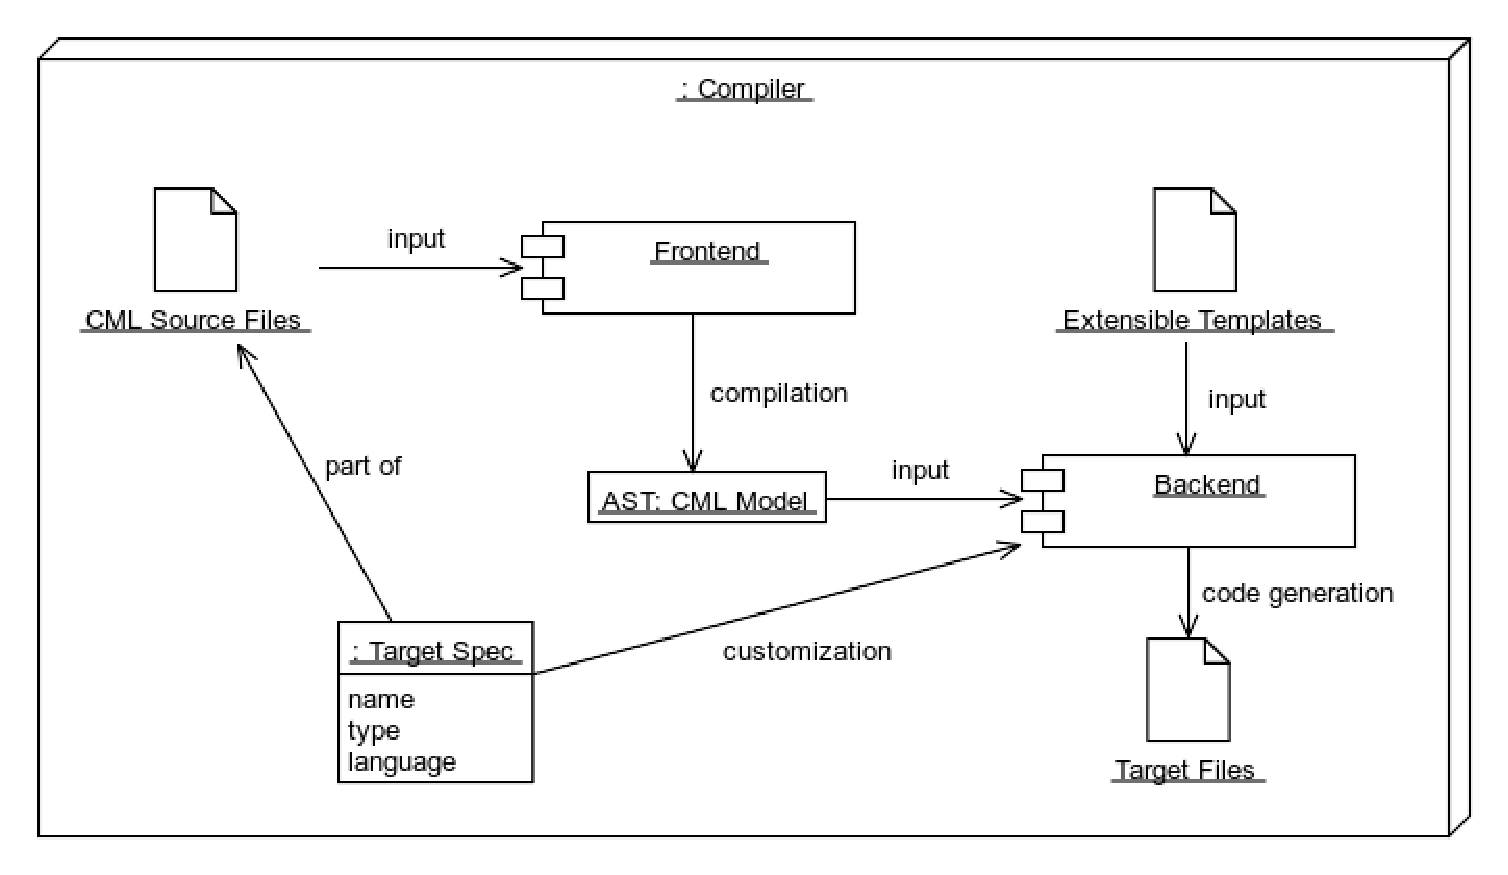
\includegraphics[width=\textwidth]{compiler/figure-overview}
\caption{An architectural overview of the CML compiler.}
\label{fig:overview}
\end{figure}

The two main components of the compiler,
and the artifacts they work with,
are presented in the next sections.

\section[Frontend]{Compiler Frontend}

Receives as input the \emph{CML source files}.
It will parse the files and generate an internal representation of the \emph{CML model}.
Syntactical and semantic validations will be executed at this point.
Any errors are presented to the developer, interrupting the progress to the next phase.
If the \emph{source files} are parsed and validated successfully, then an internal representation (AST) of the \emph{CML model} is generated.
The AST serves then as the input for the \emph{backend} component.

\section[Backend]{Compiler Backend}

Receives the \emph{CML model AST} as input.
Based on the \emph{target specification} provided by the AST, chooses which \emph{extensible templates} to use for code generation.
The \emph{target files} are then generated, and become available to be consumed by other tools. The \emph{target specification} plays a key role in order to determine the kind of \emph{target} to be generated.

CML extensible templates are implemented in StringTemplate \cite{st}.  The CML compiler uses StringTemplate for two purposes:

\begin{itemize}
\item \emph{File names and directory structure:}
each type of target generated by the CML compiler requires a different directory structure.
The CML compiler expects each target type to define a template file named ``files.stg'' (also known as \emph{files template}),
which will contain the path of all files to be generated. The \emph{files template} may use information provided by the \emph{target specification} (specified in chapter \ref{ch:targets}) in order to determine the file/directory names.
\item \emph{File content generation:}
each file listed under the \emph{files template} will have a corresponding \emph{content template} that specifies how the file's content must be generated. The \emph{content template} will receive as input one root-level element of the CML model, which will provide information to generate the file's content. The type of model element received as input by the \emph{content template} depends on which function of the \emph{files template} has defined the file to be generated.
\end{itemize}

